\chapter{绪论}

\section{分布式存储系统概述}
信息技术以及数据存储技术的发展引起了重大且深刻的社会变革,以相当程度地促进了科技的进步与发展,并且随着信息技术与数据存储技术在社会生活
中的不断渗入,电子数据的产生数量与速度都呈现着爆炸式的增长。根据IDC(International Data Corporation,国际数据公司)
预测,全球数据量将从2020年的44ZB增长到2025年的175ZB\cite{rydning2018digitization}。在如此急剧增长的数据体量面前,
传统的数据存储方式已然无法满足时代对于数据存储的需求,所以如何保证数据的安全存储以及便捷读取成为当前时代的一个非常重要的课题。

伴随着用户电子数据的不断增长和存储需求的不断增加,分布式存储系统凭借便捷性、统一性、安全性、可靠性得到了广泛的应用,
并且逐渐成为了当今信息社会的网络基础设施。分布式存储系统结合了负载均衡技术、集群技术、虚拟化技术、分布式技术、CDN加速技术,
为用户提供了数据存取的方便以及快捷且低成本的文件存储服务。

但是,目前流行的云存储系统普遍依赖中心服务器来提供云存储和数据处理服务\cite{wang2018blockchain}。
存储节点本身硬件故障或者技术原因导致的风险、设备陈旧需要替换或软件升级等原因使这些存储服务器十分容易出现短时或永久性的失效,
从而导致存储的数据永久性的丢失。例如:2018年腾讯云因磁盘故障导致文件元数据的丢失,大量的个人用户资料数据丢失;\citet{sathiamoorthy2013xoring}曾
指出“Facebook数据中心的一个大集群在一个月内的节点故障数目超过20个而一天内失效节点的数量峰值可高达100个”。
因此如何提高分布式存储系统的数据可靠性亦即数据修复技术是业界和学术界广泛关注的问题。对于可靠性低且经常发生故障的海量存储节点,
如何采用性能优越的技术和措施才能保证数据的可靠性和故障发生时如何以相对低廉的成本快速修复故障节点的数据,已然
成为了大规模分布式存储系统的重要目标和方向。

目前,分布式存储系统通常采取存储超过原本数据1.x倍的冗余数据来保证数据可靠性以对抗节点故障而导致的数据丢失,
进而通过冗余数据进行相关的计算还原出丢失的数据。分布式存储系统中冗余数据的产生方法大致可以分为两类:
\begin{enumerate}
    \item 多副本方式,即将数据对象复制多份(通常为三份),如$r$份,然后将这些副本均匀地分散到$r$个不同的存储节点上,
          当某个节点故障时,只需要从剩下任意节点中下载原文件$r-1$次,并将其重新存放到其他正常节点即可。但是在数据存储急剧增长的情况下,备份冗余会引发大量存储开销,早期的分布式集群一般采用这种方式。
          其中典型的代表有Google File System\cite{ghemawat2003google},Hadoop Distributed File System\cite{borthakur2008hdfs}等。
    \item 纠删码方式,即使用纠删码(erasure codes)技术生产冗余数据块。纠删码是通过编解码矩阵的计算创建了远小于多备份技术的冗余数据,同时提供同级别的容错性\cite{weatherspoon2002erasure}。
		  如今的大规模存储群越来越多地采用纠删码\citep{ford2010availability,huang2012erasure,muralidhar2014f4,ovsiannikov2013quantcast},进而取得存储空间和可靠性二者之间的均衡。
          具体的编码方式则是将原始文件计算分割成若干个数据块,再进行编码生成多个冗余的编码块,并将这些编码块存储到不同的节点上
          。与多副本方式相比,在存储同样体量的原始文件与同等的数据可靠性的条件下,纠删码的优点在于能够极大地节省了存储空间,
          进而减少了存储空间上的开销。目前学术界有大量的纠删码的编码方式,如Reed-Solomon码(简称RS码)\cite{reed1960polynomial},
          Regenerating Code(简称RGC码)\cite{wu2009reducing},Local Regeneration Code(简称LRC码)\cite{kamath2014codes}等。
\end{enumerate}

无论是多副本技术还是纠删码方式都会产生冗余数据,并且都有其固有的缺陷。多副本技术有着极大的存储空间开销,为了
能够容忍$(m-1)$个副本失效,而不得不额外消耗$(m-1)$倍于原始数据大小的存储空间,例如三副本机制在大数据时代,
当数据规模达到PB、EB甚至ZB级别时,多副本技术极高的存储空间成本以及维护开销将使得数据中心无法承担。除此之外,纠删码自身也存在着
相应地无法忽视的缺陷,例如修复成本过高、消耗大量的CPU资源进行编解码操作、实现过程复杂等,从而使得将该技术应用到分布式存储系统中时面临着诸多挑战。

\section{数据容错技术概述}
为了保证分布式存储系统中的数据可靠性和可用性,系统本身必须采取一定的数据容错技术。数据容错技术是指
通过某种方式对数据对象进行处理后产生的一定的冗余,并将处理后的数据发送到不同的节点上,使得如果由于某些
节点故障导致的数据失效时,能够使用剩下节点中的数据还原出丢失的数据。

为了保证系统中数据的实时可访问性,在部分数据因节点故障而丢失时必须利用健康节点上的剩余数据快速地将
数据重新恢复出来,此过程被称为“\textbf{数据修复(Data Repair)}”\cite{li2009tree}。维持数据原有
的冗余度是数据修复技术想要达到的目的,同时也要确保数据的可靠性。因为对于数据容错技术而言,能够容忍的数据
丢失是极其有限的,一旦丢失的数据超过了容错技术的容忍度,原本的数据对象将无法恢复,从而导致数据的永久性丢失。
一般的数据修复过程主要遵循以下过程:当系统检测到节点故障事件产生时,根据系统设定的容错方案开始进行启用对应的修复方案,
利用剩余的健康数据节点对丢失的数据进行恢复,再将其重新根据放置算法将数据分散存储到存活节点中去。修复时提供数据的节点称为提供节点,修复出的
数据存在的节点称为新生节点。分布式存储系统冗余机制可以分为结构容错机制和数据容错机制。

\subsection{结构容错机制}
结构容错机制实现系统容错的方式是通过提供冗余的物理设备的方法来实现的。具体的分类方式是根据冗余物理设备的
不同可以分为以下两种:基于节点冗余的冗余机制和基于链路冗余的容错机制。

基于节点冗余的容错机制实现文件冗余的方式是使用增加冗余节点的方式实现的。当系统中的某个数据节点失效以后,
系统将使用冗余节点替代失效节点\cite{ghemawat2003google,hua2009smartstore,weil2004dynamic}。

基于链路冗余的容错机制则是通过增加冗余的网络链路的方式来实现文件冗余。主要通过两种方式进行实现,其中之一为
通过在树结构的上层链路加入冗余链路来提高系统容错性\cite{al2008scalable,greenberg2011vl2},
或者通过在服务节点上添加网卡的方式实现多链路冗余\cite{guo2008dcell,guo2009bcube}。

\subsection{数据容错机制}
在传统的分布式存储系统中,用户节点通过将文件切块后再将数据块分发到存储节点中。通过创建冗余的数据编码块来
对分布式存储系统的容错能力进行提高的方式被称为数据容错机制。根据冗余数据编码块创建方式的不同,数据容错
机制可以分为基于复制的容错机制和基于编码的容错机制。
\begin{figure}[htbp]
	\centering
	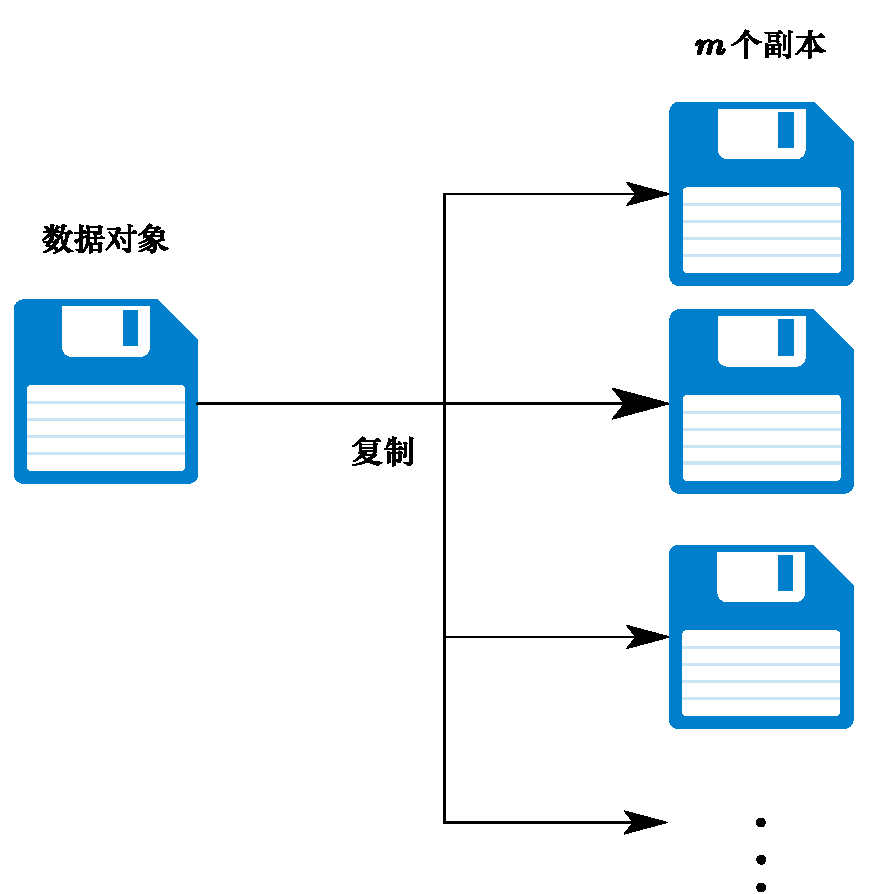
\includegraphics [scale=0.5]{figures/1.1.pdf}
	\caption{基于复制的容错机制原理}
	\label{fig:con-1.1}
\end{figure}

基于复制的容错机制原理如图~\ref{fig:con-1.1}所示,将原始数据复制多份,创建多个数据副本并分发到不同的存储节点上
从而实现数据冗余\cite{shvachko2010hadoop,ghemawat2003google,王意洁2017分布式存储中的纠删码容错技术研究}。
当一个或者多个存储着原始文件副本数据的存储节点故障时,系统通过访问其他存活节点的原始文件的副本数据,进行数据的恢复,
进而提高系统的可靠性。基于复制的冗余机制原理较为简单,易于部署和实现,并且在确保数据可靠性的基础上还能提高数据的并发访问能力。
然而,缺点显而易见,在文件储存过程中,需要分发多个多个数据副本,因此提高了数据的存储开销和通信数据的开销,存储效率较低。
对于$n$副本的复制容错机制,系统存储空间的总体利用率只有$\frac{1}{n}$。在此基础之上,为了提高存储效率,降低存储空间的开销,
可以采用动态复制机制,依据系统的网络状况、用户需求等因素进行综合考量并进行动态创建与删除副本\cite{lakshman2010cassandra,gill2016dynamic,gai2012design}。
但是,动态复制技术也存在其固有的缺陷,因为在动态创建与删除副本的过程中,需要CPU执行大量的计算,并且需要进行频繁的数据分发,从而
增加了系统的计算开销和通信开销。


相对应的,基于编码的容错机制首先对原始数据文件进行切块,再对切成的块文件进行编码,
生成体积较小的编码块从而提高数据可用性。
基于编码的容错机制生成的编码块体积小、数量少,因此,相对于基于复制的容
错机制,具有较小的存储开销。基于编码的容错机制可以分为两种:RAID技术、纠删码容错。

RAID技术\cite{patterson1988case,chen1994raid}是一种传统的基于编码的容错技术,RAID技术实现容错的方式
是通过将数据进行条带化,然后将数据条带分发到不同的存储节点上,并生成一个编码块进而实现数据的容错与冗余。
RAID技术一般只能容忍一到两个数据块的失效,因此对于大规模的分布式存储系统而言,RAID技术无法满足其数据可靠性的要求。

更加主流的基于编码的容错方式便是纠删码技术,其本身是一种编码容错技术,最早被应用到通信领域,解决数据
在传输中的纠错问题。传统的纠删码技术实现容错机制的步骤一般如下,首先将原始数据文件分割成$k$个数据块,
然后将这些数据块通过相应的矩阵计算进行编码生成$n-k$个编码块,最后将生成的$k$个数据块和$n-k$个编码块分发到
不同的存储节点中。当用户访问存储系统下载数据时,只需要从$n$个数据块中任意下载$k$个可用的块即可恢复出完整的
原始数据文件。

相较于基于复制的容错技术即多副本技术,纠删码技术最大的优势是能够以极低的存储空间开销代价换取相同甚至更高级别的
数据可靠性\cite{lin2004erasure,weatherspoon2002erasure}。例如,RS(12, 10)码可以凭借0.2倍的额外存储空间开销
获取两个节点的容错能力,这比具有同等容错能力的三副本技术节省了约60\%的存储空间。在同等的存储空间利用的情况下,
以纠删码技术构建的分布式系统的数据可靠性比采用多副本技术构建的分布式存储系统中的数据可靠性要大几个数
量级\cite{lin2004erasure,weatherspoon2002erasure}。
尽管有很多代表性的工作\citep{huang2019lower,xu1999x,reed1960polynomial,roth1989mds}对于纠删码的计算性能进行了优化,
但是纠删码方案由于其固有的缺陷如大量的矩阵计算编解码操作,依然会产生巨大的通信开销。因此如何提高纠删码容错的效率是一个亟需解决的重要问题。

\section{纠删码概述}
近年来,越来越多的大规模存储系统采用了具有较强容错能力和空间利用率较高的纠删码实现系统冗余\citep{xia2007robustore,kubiatowicz2000oceanstore}。
随着时代发展,数据规模越来越大,如何提升纠删码的容错能力用以满足系统的存储和访问需求已然成为学界与业界广泛关注的问题。

纠删码的主要思想是把一个数据对象$D$分为$k$个相同大小的数据块,通过一定的矩阵计算和编码算法生成
$n$个块($n>k$),使得通过其中任意$k'$个块即可重新还原出原始数据,具体过程如图~\ref{fig:con-1.2}所示。

\begin{figure}[htbp]
	\centering
	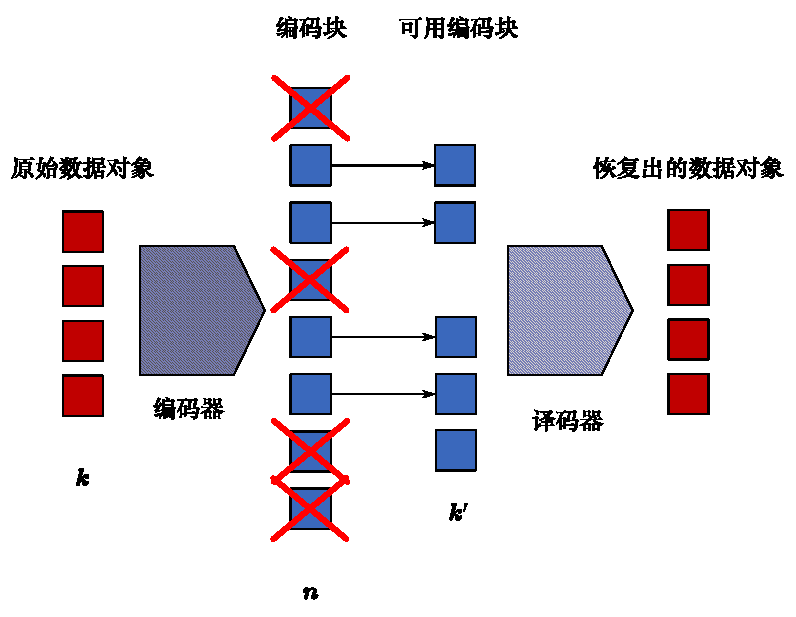
\includegraphics [scale=0.8]{figures/1.2.pdf}
	\caption{纠删码编码和解码示意图}
	\label{fig:con-1.2}
\end{figure}







一般来说,纠删码可以用三元组$(n,k,k')$表示。其中$k$是数据切分成的数据块个数,$k'$是一个不小于$k$的数,
$n$是编码后的块数。首先,将数据对象$D$分割成$k$个大小相等的数据块$D_1,D_2,...,D_k$,然后通过
编码算法和矩阵运算将这$k$个数据块进行编码,生成$n$个同等大小的编码块$I_1,I_2,...,T_n,n>k$,使得
通过其中任意$k'$个块都能还原出原始的数据对象$D$的对应的$k$个数据块$D_1,D_2,...,D_k$,从而组合出原始的数据。
纠删码可以容忍的最多失效块的个数称为容错度,当$k=k'$时,纠删码达到理论上的最高容错力,称之为最大距离可分码
(Maximum Distance Separable,简称MDS码)\cite{blaum1996mds}。这样的纠删码可用二元组
$(n,k)$表示,如果纠删码生成的$n$个块集合中包含全部的$k$个原数据块,这样的纠删码便是系统码(System Code)\cite{plank2009raid}。
对于系统码而言,编码后生成的额外$n-k$个块称为编码块,并且记为$P_1,P_2,...,P_m$,其中
$m=n-k$。如果数据块没有丢失,应用系统码的存储系统在相应数据访问操作时无需进行解码操作,性能大大提升,这也是现有的纠删码大多是系统码的原因。

在存储系统实际的运行过程中,先将文件分割成固定大小的数据块,再将这些数据块每$k$个作为一组,每组
独立进行编码操作生成$n$个块,其中$n$个块的集合称为一个条带(Stripe)\cite{hafner2005matrix},
$k$称为条带长度(Stripe Length)。当数据对象的块数不是$k$的整数倍或者最后一个数据块不足一个整块时,以0填充,被0填充的部分不需要存储在真正的磁盘上,
在数据修复时也不需要读取。根据计算方式和几何构造的不同,纠删码可分为Reed-Solomon码、阵列结构型纠删码、
网络编码型纠删码和分组结构型纠删码。

\subsection{Reed-Solomon码}
Reed-Solomon码\cite{reed1960polynomial}是最为经典的MDS码,是唯一可以用任意的数据磁盘数目和任意冗余磁盘
数目的MDS码。RS码的编码原理是通过矩阵的运算来完成的,如果分布式存储集群采用的是结构为
$(k+r,r)$的RS编码,则整个分布式存储集群应具有$k$个数据块和$r$个编码块。
在基于RS编码的分布式存储集群中,如图~\ref{fig:con-1.3}所示,编码块是通过将$k$个数据块
与$k\times (k+r)$个生成矩阵相乘来构造的,该生成矩阵主要包含了两个变量,一个
$k \times k$校验矩阵和一个$k \times r$冗余矩阵\cite{li2016procode}。一个由$(k+r,r)$
组成的RS编码存储集群,含有$k+r$个存储节点的阵列,其中$k$个数据块和$r$个编码块分别存储在存储集群中的
$k$数据节点服务器和$r$个奇偶校验节点服务器上。

\begin{figure}[htbp]
	\centering
	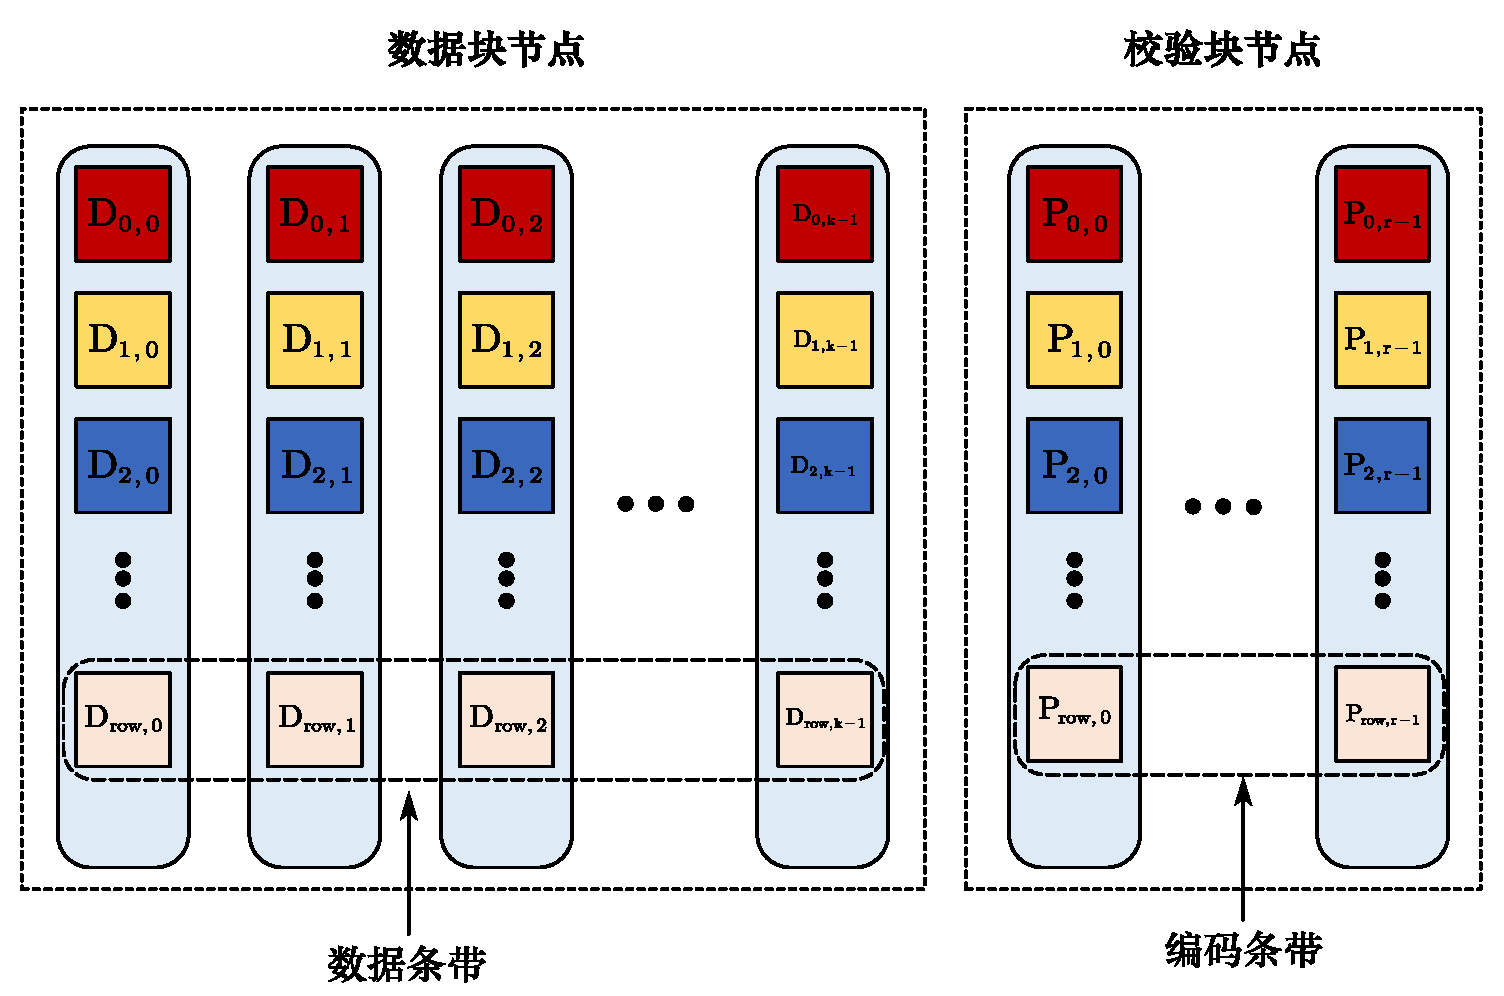
\includegraphics [scale=0.5]{figures/1.3.pdf}
	\caption{传统基于RS码结构的存储集群布局}
	\label{fig:con-1.3}
\end{figure}

RS码实际上是利用生成矩阵和数据列向量进行矩阵乘法得到编码列向量。
RS码使用的生成矩阵$G$中的任意$k$行组成的矩阵需要在Galois域上可逆,故获得生成矩阵的计算量并不低,且可由范德蒙德(Vandermonde)矩阵或柯西(Cauchy)矩阵\cite{roth1989mds}通过变换得到。
采用前者计算方法的RS码称为范德蒙德RS码,采用后者计算方法的RS码称为柯西RS码。在Galois域上,加法的定义是异或运算,
乘法则需要使用离散对数运算和查表,因此计算开销很大,而应用柯西矩阵可将乘法运算转化为二进制
的乘法运算,从而减轻运算量。

RS码拥有比传统多副本容错更高的容错能力和更高的灵活性。RS码不仅达到了理论上的最高
容错能力,而且其条带长度$k$可以取任何大于0的整数,编码后产生块数$n$可以
取任何大于$k$的整数。$n$相对于$k$越大,RS码的容错能力越高,但存储空间消耗
也越多。因此,RS码在可靠性和存储空间开销方面给予了系统很大的选择空间。

然而,纠删码的其中一个弊端在于会引起大量的带宽以及计算资源的消耗,进而导致存储效率的降低。由于计算能
力的限制,RS码从诞生起其编解码算法就已被广泛研究和优化,计算复杂
度高的问题已被较好地解决。近年来各种硬件的计算能力的显著提升,在分布式存
储系统中进行编解码运算并不会占用过多的计算资源。与RS码在信道中纠错时不
同,当RS码作为分布式存储系统的数据容错技术时,由于其产生的$n$个编码块必
须分别放在$n$个不同的节点上,若只有一个丢失,在进行数据修复时也需
要从不同节点下载$k$个编码块。这是多副本技术中修复一个块需要数据量的$k$
倍,会占用大量的网络资源,并极大地降低了修复速度。

RS码高昂的修复成本使其在分布式存储系统中的应用有很多亟待解决的问题。
然而,RS码高容错和低空间消耗的优点对提高分布式存储系统的数据可靠性和降
低其经济成本具有重大意义。为了解决这一问题,涌现出了众多修复成本较低的纠
删码。这些低修复成本的纠删码根据其采用的基本技术可以分为三类:基于阵列结构的纠删码
、基于网络编码的纠删码和基于分组结构的纠删码。

\subsection{基于阵列结构的纠删码}
阵列码是一种采用阵列结构编码且完全基于异或运算的纠删码,从
冗余磁盘阵列(RAID)\cite{patterson1988case}技术中不断发展出来。
阵列码的含义就是将原始的数据和冗余的数据一起存储在一个二维的阵列中。
根据数据块和编码块放置方式的不同,阵列码可以分为横式阵列码和纵式阵列码。

横式阵列码(horizontal parity array codes)的特点是将数据块和相应的编码块分发到不同的数据节点上。
它的结构特点是将冗余的数据单独放到独立的磁盘中,这些磁盘也被称为冗余磁盘,
而让别的磁盘专门用于存储数据,这样做的好处是可扩展性很强。


EVENODD编码\cite{blaum1995evenodd}是最早被发表的阵列码,EVENODD码的编码块和数据块之间的计算关系
如图~\ref{fig:con-1.4}所示。其中第一列上的编码块分别由各自同一行上的其他数据块进行异或得到,
第二列上的编码块由与其直线相连的对角线上的数据块进行异或运算得到。此外,RDP\cite{corbett2004row}编码也是
一种应用较为广泛的横式阵列码,这些编码体系均对磁盘数目提出了严格的要求(要求磁盘数目必须是素数或者素数减1),
同时还要求在单个条带中的数据元素的个数必须与磁盘的数目相匹配。

除了EVENODD和RDP,其他的横式阵列码有EEO\cite{feng2010eeo},
STAR\cite{huang2008star},
RAID-6 Liberation\cite{plank2009raid}和Feng's Code\cite{feng2005new}等,
它们具有性能比较优秀的编码效率和极高的存储空间利用率。由于横式阵列码本身固有的缺陷,如写入数据总会用到冗余磁盘,
故其中的I/O流量成为了横式阵列码的性能瓶颈。


\begin{figure}[htbp]
	\centering
	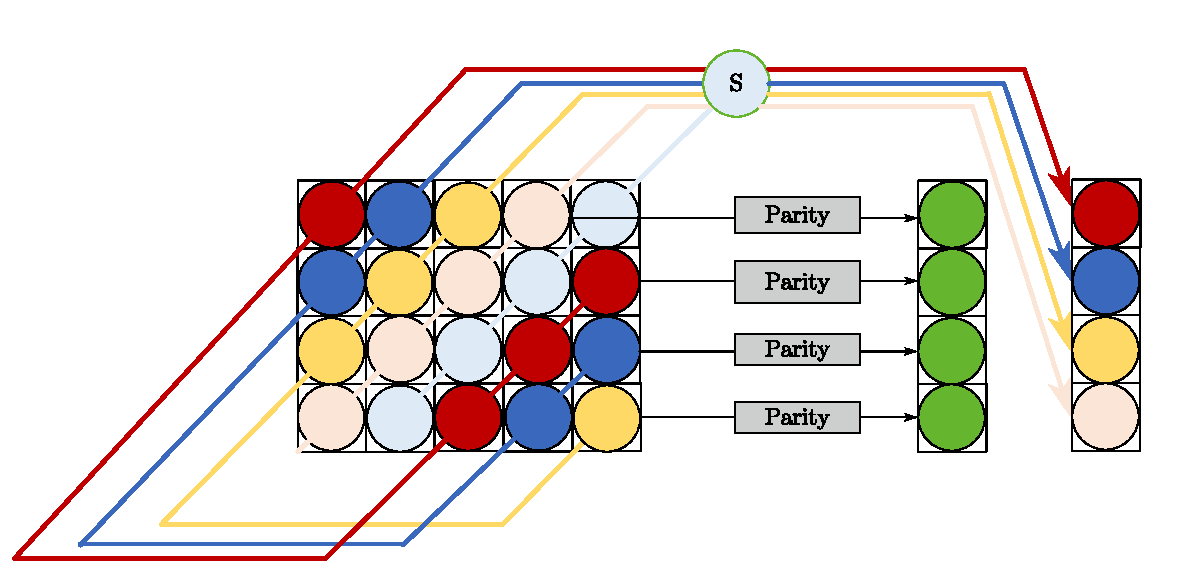
\includegraphics [scale=0.7]{figures/1.4.pdf}
	\caption{EVENODD码的编码结构示意图}
	\label{fig:con-1.4}
\end{figure}

纵式阵列码(vertical parity array codes)是指冗余存储在数据条带中的阵列编码方式,即冗余数据和原始数据
混合放在磁盘中的纠删码。由此可以看出纵式阵列码将计算工作和写入操作均匀地分摊到各块磁盘上,从而实现了
负载均衡。X-code\cite{xu1999x}是具有MDS性质的纵式纠删码,其在编码操作,数据更新以及数据重构等步骤上具有
理论上的最优效率,缺点就是可扩展性比较差。


X-code的编码方法如图~\ref{fig:con-1.5}所示,同一列上的数据块与编码块表示存储在同一个存储节点中,
存储节点上包含$k$个编码块。其中红色块代表数据块,蓝色块代表编码块,$n$需要是一个大于2的素数,数据个数必须
为$n-2$个,编码块的个数也必须是2个。此外,第一个编码块由主对角线上的数据块进行计算得到,另外一个编码块由副对角线
的数据块计算得到,这些计算需要用到$k$个磁盘上的数据块,计算成本较高,且修复时需要按照一定的顺序进行计算,失去了并行
修复的可能,这些均是X-code的不足之处。

\begin{figure}[htbp]
	\centering
	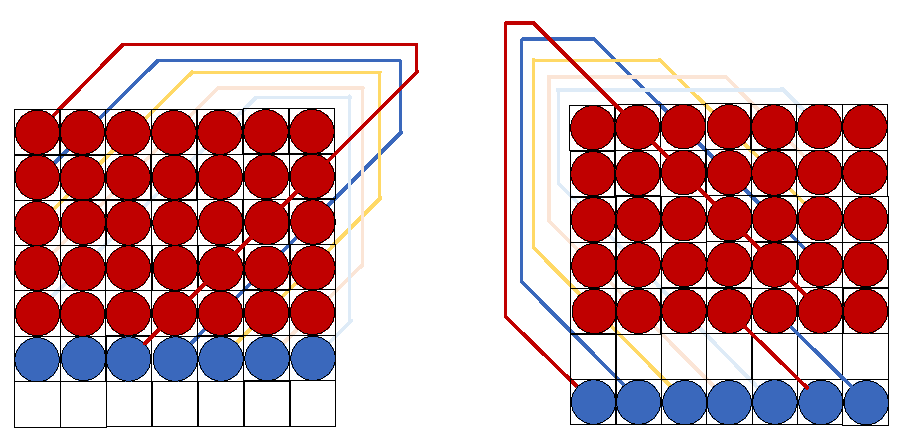
\includegraphics [scale=0.7]{figures/1.5.pdf}
	\caption{X-code的编码结构示意图}
	\label{fig:con-1.5}
\end{figure}


阵列码在计算上的主要特点就是所有的运算都是异或运算,相较于传统的RS编码在计算性能上有优化,但需要的数据量却并没有
丝毫减少,传输的数据量较大。


\subsection{基于网络编码的纠删码}
网络编码最初由\citet{ahlswede2000network}于2000年首次提出。
在传统的网络路由中,中间节点只具备存储和转发的功能。
而网络编码则增强了中间节点的功能,使得其不仅可以
存储转发数据,并且还可以在转发数据之前对数据进行编码和组合计算,从而
减少了网络中的数据传输量并提高了网络吞吐率。

\citet{dimakis2010network}将网络编码的思想应用到纠删码上并称之为再生码
(Regenerating Codes)。
再生码允许新生节点访问多于$k$个节点,从而显著降低修复过程需要传输的总数据
量。


\begin{figure}[htbp]
	\centering
	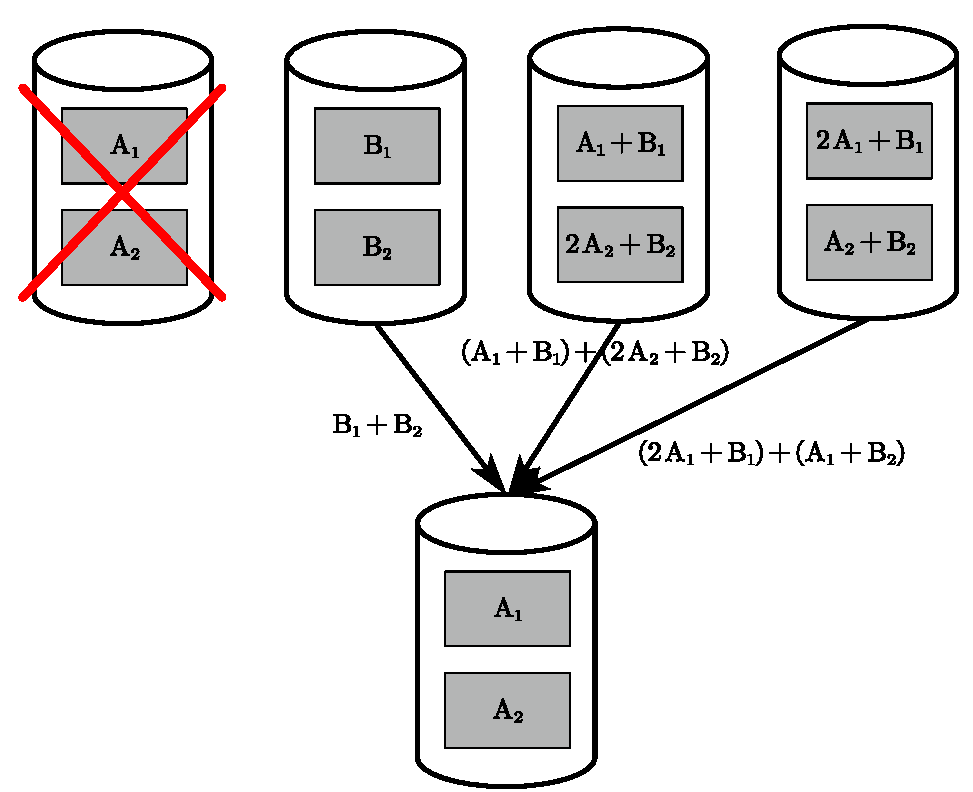
\includegraphics [scale=0.6]{figures/1.6.pdf}
	\caption{再生码修复失效数据节点示意图}
	\label{fig:con-1.6}
\end{figure}

图~\ref{fig:con-1.6}显示了再生码修复失效数据节点过程,总共有四个用来存储数据的节点,
并且每个存储
节点上存放着两个数据块,并且是通过相关的矩阵运算生成的。
若第一个存储节点发生故障时,则相应的存储的数据块会丢失。
针对此种情况,传统纠删码的修复方法是在剩下的三个存储节点中任选两个,
将这两个节点的所有数据块发送给新生节点(newcomer)
,传输数据块的总数目为4。
而再生码的思想是首先在存储节点中进行相应的计算后再进行数据分发,
传输数据块的总数目为3,相较于传统的修复方法,再生码修复数据传输量降低
了25\%。


\citet{dimakis2010network}提出的再生码可以对丢失的数据进行精确修复,
但对编码块只能进行功能性修复。
所谓功能性修复,亦即修复出的数据与原来的冗余数据并不是一模一样的,但却可以维持数据的容错度不变。
针对此问题,
\citet{wu2007deterministic}提出了确定性再生码
(Deterministic Regenerating Codes),并从概率学角度证明了其存在性。

根据存储效率的不同,再生码可以分为$\frac{k}{n}\leqslant \frac{1}{2}$的低比特率码和
$\frac{k}{n}> \frac{1}{2}$的高比特率码。它们可以在一定程度上从源头减少修复过程中传输的数据量,
但是由于编码系数所在域的要求限制和选择方法的不规则,难以实现等原因,目前应用并不广泛。


\subsection{基于分组结构的纠删码}
基于分组结构的纠删码可以减少数据修复时需要下载的数据量,因传统的RS码在修复一个丢失的块时
需要下载的数据条带长度为$k$,而分组结构的纠删码的方法则是将$k$减小从而达到降低数据量的目标。
分组编码的纠删码首先将数据条带分成若干组,各个组各自计算相应的编码块,实现组内修复丢失块,需要的块数
则取决于每个组内的数据块数。而相应的,RS码作为一种特殊的分组编码,将整个数据条带作为一组,此外根据
分组方法的不同,此类纠删码可以分为两类:水平分组结构的纠删码和交叉分组结构的纠删码。

比较经典的水平分组纠删码一般是将数据条带分为两组。每个小组生成一个局部的冗余块,然后整个条带
再生产一个全局的冗余块。这样数据修复就可以依靠小组内的编码块完成,降低了修复成本。图~\ref{fig:con-1.7}显示的是微软的
Azure系统\cite{calder2011windows}采用LRC(Local Reconstruction Codes)\cite{huang2012erasure}
的一个实际的例子LRC(8,2,2)。可以看出,它将数据块平均分为了两组,每组各自内部计算出一块局部冗余编码块,
相当于一个RS(5,4)码。对于两个条带再生成2个全局的校验块,则相当于一个RS(10,8)码。当丢失块数不多时,如1个则只需要4个块即可进行数据修复,
这样就有效降低了修复成本。

\begin{figure}[htbp]
	\centering
	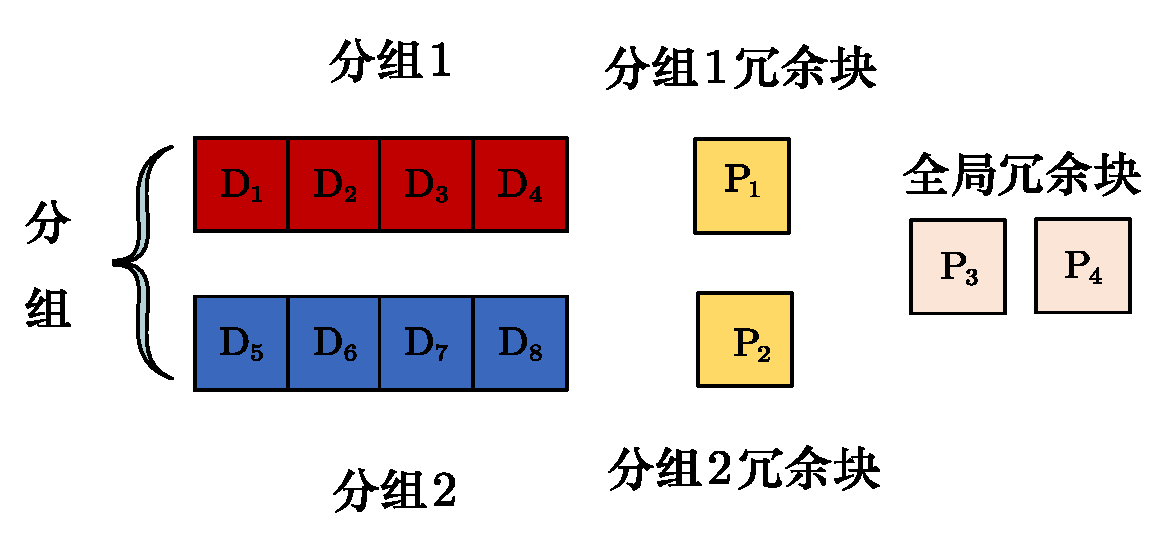
\includegraphics [scale=0.5]{figures/1.7.pdf}
	\caption{LRC(8, 2, 2)的编码示意图}
	\label{fig:con-1.7}
\end{figure}

由此可以发现,组数越多,那么可以容忍的失效的块数也就越多,故Pyramid码\cite{huang2013pyramid}便诞生了,
它的特点就是可以对条带内的数据块进行任意层次的分组,层次越多平均的修复成本也就越低,但是相对的存储空间消耗也就越大,
因为产生了更多的全局校验块,对于Pyramid码需要根据实际的存储系统环境选择更加适中的方案。除此以外水平结构
的编码还有运行在Facebook旗下的分布式存储系统中的XORing Elephants\cite{sathiamoorthy2013xoring}、
EXPyramid\cite{周松2011expyramid}、LRCs\cite{sathiamoorthy2013xoring}等。EXPyramid码是对两层
Pyramid码的一种改进,其分为了三组。

交叉分组结构的纠删码与水平分组不同之处大致有两点。第一,交叉分组纠删码的分组方式不同,交叉分组
的各组之间相互重叠但却互不包含,相比之下水平分组各组之间一般不重叠且会有一个全局的校验块包含着各个分组的校验块。
第二,交叉分组纠删码编码计算较为简单,基于异或计算。不难看出,交叉分组有着相对来说较低的计算性能消耗的优点。常见的交叉结构的
纠删码有\citet{woitaszek2007tornado}提出的Tornado码,如图~\ref{fig:con-1.8}所示,其任何组别的冗余块均为组内的数据块的校验块,并且
修复任何一个数据块或者冗余块只需4个或3个块,避免了大量下载编码块的特殊情况。此外还有
LDPC\cite{gallager1962low}、WEAVER码\cite{hafner2005weaver}和Tanner码、Hover码\cite{hafner2006hover}等。

\begin{figure}[htbp]
	\centering
	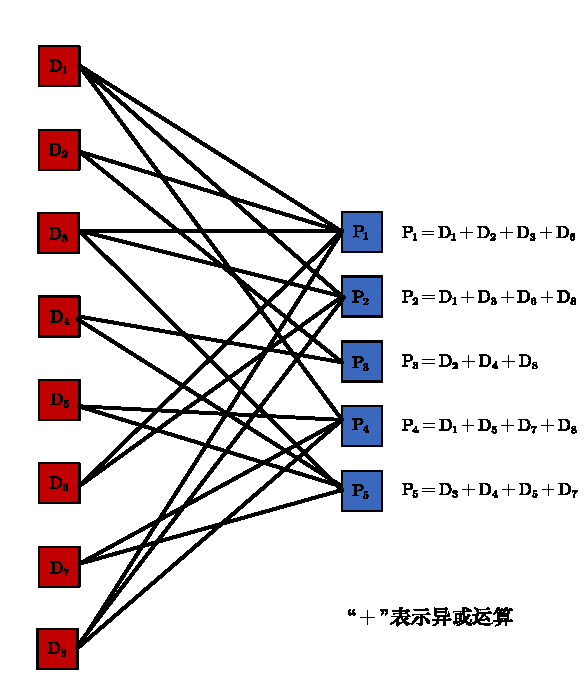
\includegraphics [scale=0.7]{figures/1.8.pdf}
	\caption{Tornado码的构造示意图}
	\label{fig:con-1.8}
\end{figure}

\section{基于纠删码的数据修复技术}
在基于纠删码的分布式存储系统中,数据传输并不是简单的线性路线,修复一个丢失的数据块时,
提供者节点要向新生节点传输多个数据块用以完整地修复数据,数据的传输路径往往比较多样化,根据传输
路径的不同一般可分为三种修复技术:基于星型拓扑的数据修复、基于树型拓扑的数据修复和基于XOR的纠删码数据修复。

\subsection{基于星型拓扑的数据修复}
基于星型拓扑的串行修复技术(Star Structure Based,SSR)是指依序逐个修复故障的节点数据,每个故障
节点的修复过程都是按照星型拓扑来进行的。具体来说,以新生节点为中心,各个存活节点之间并不相互传输数据,
存活节点直接向新生节点传输数据,从而形成了一个以新生节点为中心、存活节点为边界的星型拓扑结构。
可以看出,修复的时间取决于新生节点与存活节点之间最慢的一条带宽链路。

\citet{dimakis2010network,wu2007deterministic}提出的再生码数据修复过程要求每个存活节点向
新生节点传输均等的数据量进行修复,数据收集节点(DC节点)仅连接$k$个节点,通常
是$k-1$个数据节点和第一个校验数据节点,并从每个节点下载$\frac{M}{k}$的数据量($M$为原文件大小)。这里存在一个
非常明显的缺陷,节点可以选择的链路比较单一,带宽较高的链路很有可能会被忽视,导致修复效率降低。
\citet{shah2010flexible}提出了弹性修复的方法,即允许存活节点和DC节点充分利用所有可用的链路,
从中选择带宽较大的链路进行数据传输,传输的数据不均等。DC节点从节点$i(1 \leqslant i \leqslant n)$
下载$\mu_i (0 \leqslant \mu_i \leqslant \alpha)$,满足总下载量不小于$M$即可。同理,新生节点从存活节点
$i(1 \leqslant i \leqslant n)$接收$\beta_i (0 \leqslant \beta_i \leqslant \beta_{max})$
数据量,满足总接收量大于或等于一个设定参数$\gamma$即可,用不等式表示
则如~\ref{eq:1-1}和~\ref{eq:1-2}:

\begin{equation}
	\label{eq:1-1}
	\sum_{i=1}^{n} \mu_{i} \geq M, 0 \leq \mu_{i} \leq \alpha
\end{equation}
\begin{equation}
	\label{eq:1-2}
	\sum_{i=1}^{n} \beta_{i} \geq \gamma, 0 \leq \beta_{i} \leq \alpha
\end{equation}

当一个节点故障时,新生节点可以选择任意$k$个节点下载$\frac{M}{k}$的数据量,修复带宽相等于原文件大小。
对于弹性修复方法而言,新生节点,可以根据可用带宽的大小从不同节点上下载不均等的数据来降低修复时间。
当然星型拓扑的缺点也很明显,DC节点需要收集多个节点的数据,修复速度会受到磁盘和网络I/O的限制,编解码的计算消耗也很大。

\subsection{基于树型拓扑的数据修复}
上节所描述的星型拓扑的技术其实是树型拓扑修复技术的特殊情况,然而修复速度受到了诸多的制约,为了提升修复的速度,
树型拓扑修复方法因此被提出。

\citet{li2009tree,li2010tree}独辟蹊径地首次设计了一个新的基于网络带宽的树形修复方法(Tree-structured Data Regeneration),
利用木桶原理并通过提高最低传输速度来加速数据的修复。这种修复方法中数据的传输路径称为修复树,修复树中所有节点都由提供者节点
(Providers)和新生节点(newcomer)组成。提供者节点可接收别的提供者节点发来的数据并将其与本节点存
储的数据进行计算,并将计算结果发给另一个提供者节点或新生节点。经证明,最大生成树是基于网络带宽的最优的修复树。

基于网络带宽的树形修复方法在一定程度上缓解了星型修复时新生节点由于同时接收大量
数据造成网络拥堵。传统的星型修复中新生节点因为承担所有计算任务而导致负载重,
而基于带宽的树形修复会将计算负载均衡到各节点,从而避免了此问题。最后,基于网络带宽的树形修
复方法使得修复任务流水化,提高修复速度。但是基于带宽的树形修复的缺点
也显而易见,由于带宽的实时动态变化速度很快,导致网络带宽不好测量或测量结果不准确,
所以此方法在网络带宽不稳定的环境下有一定的局限性。

另一类树形结构的修复技术是基于网络拓扑的树形修复技术,最具代表性是
NTar\cite{许方亮2013ntar}。NTar考虑了两种因素,包括网络上传输的数据量和数据传输过程中的网络距
离。网络距离指的是两个节点之间的物理链路数目,单位为跳
(Hop)。这种技术将修复操作对系统资源的占用看做是修复过程传输的
数据量和这些数据经过的交换设备数目的乘积。相较于传统的树形修复技术,单
纯地用数据流量来衡量修复操作对系统资源的占用情况,基于网络拓扑的树形修
复方法可以更精确地反映出数据传输对交换设备产生的影响。

在应对多节点失效时,现有的分布式存储系统采取的方法是顺序、独立地执
行多个单节点修复过程。这样不仅造成多节点修复速度缓慢,而且还造成多节点
修复时网络拥堵情况,严重影响了系统性能。为此,研究者们提出了基于树形结
构的并行修复技术\cite{weidong2013tree}。基于树形结构的并行修复技术分为分离边策略和共享边策
略。所谓分离边策略是指在同时构建修复树时,各个修复树的边不能在网络拓扑
中重合。分离边策略的初衷是尽量让多个修复树使用不同的网络链路,从而充分
利用网络资源,但此策略存在两个问题。第一个问题是为了让不同修复树中的边
不重叠,在构建一个修复树之后就将此树的所有边从网络拓扑图中删除,后续构
建的修复树只能基于剩下的网络拓扑图。这样做的后果是网络拓扑图中边变得越
来越少,如果同时需要构建的修复树数目足够多的话,将会出现无法继续构建有
效修复树的情况。第二个问题是,即使拓扑结构中两个节点之间的网络带宽被前
面的修复树占用了一部分,但剩余的空闲带宽仍可以很大。这时,如果将此条网
络路径从网络拓扑中删除,将导致后续的修复树无法构建最优的修复树。为了解
决上面两个问题,研究者们又提出了共享边的树形修复策略。顾名思义,共享边
的数据修复策略在构建多个修复树时,不同修复树之间的边可以在网络拓扑中重
合。此策略相比于分离边策略更加灵活,且实际效果更好。


\subsection{基于XOR的纠删码数据修复}

\citet{xiang2010optimal}提出的基于异或运算(XOR)的纠删码低网络负载数据修复技术
,专门用于优化RDP码\cite{corbett2004row}
修复失效数据所传输的数据量。\citet{khan2012rethinking}将其一
般化,使其适用于任何基于异或运算的纠删码。基于异或运算的纠删码在编码之前,
将每一个数据块分割成若干个大小相等的数据片(segment)
,按照某个具体的编码规则编码产生编码块,同样,每个编码块也是由若干个编码片组成,每个编码块中的各编码片
经过几个数据片异或运算而产生。目前有三种比较主流的基于异或运算的纠删码数据修复方
法,分别是提高降级读性能的EG算法修复方法、降低修复时间的 
PHR算法修复方法和降低修复成本的CHR算法修复方法。

提高降级读性能的EG算法修复方法针对的是降级读情况下的修复。节点失效的类型有两种,分别为永久失效和暂时失效,永久失效一般是指节点存储的数据丢失
了,暂时失效是指节点存储的数据只是暂时不能读但依然还存储在系统中。对于前一种失效情况,系统进行失效修复(failure recovery),
对于后一种,系统进行降级读(degrade read),
降级读操作既要读可用数据,也要读不可用的数据,如果需要读不可用数据时,系统要进行相应数据的恢复操作。
使用纠删码方式是通过矩阵计算的方式进行,当单个节点失效时,可用节点存储的编码块仍然可以用一个编码子矩阵表示,恢复数据的过程
就是计算相应解码子矩阵的过程。针对节点带宽的异构性,\citet{zhu2014boosting}提出了枚举贪心算法(Enumerated Greedy Algorithm),简称 
EG算法,EG算法遍历所有$d$个可用节点可能的组合,在每一种组合下有$l$个CDREs,计算每个CDREs的降级读时间,更新
降级读时间,使每个块的降级读时间最小。

降低修复时间的PHR算法修复方法。\citet{niu2013phr}提出了针对RAID-6编码系统中的多条带修复策略。这种策略将单个条带的修复过程分为了三个部分:
读数据、编解码、写入数据。与此同时考虑了I/O并行性和节点的异构性,提出了并行异构恢复算法(parallel heterogeneous recovery),简称
PHR算法,并且该算法能及时返回一个最优修复序列。应用PHR算法进行单条带数据修复时,三个阶段分别如下:1)得到PHR算法输出的序列,从可用的磁盘上读取
相应的数据和校验对象;2)对读取到的对象进行解码得到丢失的对象;3)将得到的对象写入其他健康磁盘上。虽然三个阶段是按顺序执行的,但是由于各条带的修复
过程的相对独立性,可以通过多线程和流水线修复技术并行化修复过程,从而达到减少降级读的时间。

降低修复成本的CHR算法修复方法。对于一条链路上由于节点之间的带宽速度的不同而造成的传输一个元素的成本差异,\citet{zhu2012cost}将传输成本
和带宽资源联系起来,定义修复总成本为$\mathrm{C}=\sum_{i=0, i \neq k}^{p} w_{i} y_{i}$,,其中假设节点$k$失效,$w_i$表示从节点$i$读取一个
对象的成本,$y_i$表示从节点$i$读取的对象数目,进而他们提出了基于传输成本的异构恢复(cost-based heterogeneous recovery)算法,简称CHR算法。
CHR算法所有的最小读取量恢复序列进行枚举,并且计算这些序列的修复成本的总和,返回其中最小的总修复成本对应的修复序列。


\section{纠删码及修复技术的问题和挑战}

\section{论文主要研究内容}

\section{论文组织结构}

